\chapter*{Introduction}
\phantomsection
\addcontentsline{toc}{chapter}{Introduction}

The purpose of this Book is the elementary study of the infinitesimal properties of one real variable; the extension of these properties to functions of several real variables, or, all the more, to functions defined on more general spaces, will be treated only in later Books.

The results which we shall demonstrate will be useful above all in relation to (finite) real-valued functions of a real variable; but most of them extend without further argument to functions of a real variable taking values in a topological vector space over R (see below); as these functions occur frequently in Analysis we shall state for them all results which are not specific to real-valued functions.

The notion of a topological vector space, of which we have just spoken, is defined and studied in detail in Book V of this Series; but we do not need any of the results of Book V in this Book; some definitions, however, are needed, and we shall reproduce them below for the convenience of the reader.

We shall not repeat the definition of a vector space over a (commutative) field K (Alg., II, p.~193). \(^{1}\) A topological vector space E over a topological field K is a vector space over K endowed with a topology such that the functions \(x + y\) and xt are continuous on \(E \times E\) and \(E \times K\) respectively; in particular, such a topology is compatible with the structure of the additive group of E. All topological vector spaces considered in this Book are implicitly assumed to be Hausdorff. When the topological group E is complete one says that the topological vector space E is complete. Every normed vector space over a valued field K (Gen.~Top., IX, p.~169) \(^{2}\) is a topological vector space over K.

Let E be a vector space (with or without a topology) over the real field R; if x, y are arbitrary points in E the set of points \(\mathbf{x}t + \mathbf{y}(1 - t)\) where t runs through the closed segment {[}0, 1{]} of R is called the closed segment with endpoints x, y. One says that a subset A of E is convex if for any x, y in A the closed segment with endpoints x and y is contained in A. For example, an affine linear variety is convex; so is any closed segment; in \(R^{n}\) any parallelotope (Gen.~Top., VI, p.~34) is convex. Every intersection of convex sets is convex.

We say that a topological vector space E over the field R is locally convex if the origin (and thus any point of E) has a fundamental system of convex neighbourhoods. Every normed space is locally convex; indeed, the balls \(\|x\| \leqslant r (r > 0)\) form a fundamental system of neighbourhoods of 0 in E, and each of these is convex, for the relations \(\|x\| \leqslant r\) , \(\|y\| \leqslant r\) imply that

\[
\| \mathbf {x} t + \mathbf {y} (1 - t) \| \leqslant \| \mathbf {x} \| t + \| \mathbf {y} \| (1 - t) \leqslant r
\]

for \(0 \leqslant t \leqslant 1\) .

Finally, a topological algebra A over a (commutative) topological field K is an algebra over K endowed with a topology for which the functions \(x + y\) , xy and xt are continuous on \(A \times A\) , \(A \times A\) and \(A \times K\) respectively; when one endows A only with its topology and vector space structure over K then A is a topological vector space. Every normed algebra over a valued field K (Gen.~Top., IX, p.~175) is a topological algebra over K.

\chapter{Derivatives}

\section{FIRST DERIVATIVE}

As was said in the Introduction, in this chapter and the next we shall study the infinitesimal properties of functions which are defined on a subset of the real field \(\mathbf{R}\) and take their values in a Hausdorff topological vector space \(E\) over the field \(\mathbf{R}\) ; for brevity we shall say that such a function is a vector function of a real variable. The most important case is that where \(E = \mathbf{R}\) (real-valued functions of a real variable). When \(E = \mathbf{R}^n\) , consideration of a vector function with values in \(E\) reduces to the simultaneous consideration of \(n\) finite real functions.

Many of the definitions and properties stated in chapter I extend to functions which are defined on a subset of the field C of complex numbers and take their values in a topological vector space over C (vector functions of a complex variable). Some of these definitions and properties extend even to functions which are defined on a subset of an arbitrary commutative topological field K and take their values in a topological vector space over K.

We shall indicate these generalizations in passing (see in particular I, p.~10, Remark 2), emphasising above all the case of functions of a complex variable, which are by far the most important, together with functions of a real variable, and will be studied in greater depth in a later Book.

\subsection{DERIVATIVE OF A VECTOR FUNCTION}

DEFINITION 1. Let \(\mathbf{f}\) be a vector function defined on an interval \(\mathbf{I} \subset \mathbf{R}\) which does not reduce to a single point. We say that \(\mathbf{f}\) is differentiable at a point \(x_0 \in \mathbf{I}\) if

\(\lim_{x\to x_{0},x\in I,x\neq x_{0}}\frac{\mathbf{f}(x)-\mathbf{f}(x_{0})}{x-x_{0}}\) exists (in the vector space where f takes its values); the

value of this limit is called the first derivative (or simply the derivative) of f at the point \(x_{0}\) , and it is denoted by \(\mathbf{f}'(x_{0})\) or \(\mathbf{D}\mathbf{f}(x_{0})\) .

If f is differentiable at the point \(x_{0}\) , so is the restriction of f to any interval \(J \subset I\) which does not reduce to a single point and such that \(x_{0} \in J\) ; and the derivative of this restriction is equal to \(\mathbf{f}'(x_{0})\) . Conversely, let J be an interval contained in I and containing a neighbourhood of \(x_{0}\) relative to I; if the restriction of f to J admits a derivative at the point \(x_{0}\) , then so does f.

We summarise these properties by saying that the concept of derivative is a local concept.

Remarks. *1) In Kinematics, if the point \(\mathbf{f}(t)\) is the position of a moving point in the space \(\mathbf{R}^3\) at time \(t\) , then \(\frac{\mathbf{f}(t) - \mathbf{f}(t_0)}{t - t_0}\) is termed the average velocity between the instants \(t_0\) and \(t\) , and its limit \(\mathbf{f}'(t_0)\) is the instantaneous velocity (or simply velocity) at the time \(t_0\) (when this limit exists).*

\begin{enumerate}
\def\labelenumi{\arabic{enumi})}
\setcounter{enumi}{1}
\tightlist
\item
  If a function \(\mathbf{f}\) , defined on I, is differentiable at a point \(x_0 \in I\) , it is necessarily continuous relative to I at this point.
\end{enumerate}

DEFINITION 2. Let \(\mathbf{f}\) be a vector function defined on an interval \(\mathrm{I} \subset \mathbf{R}\) , and let \(x_0\) be a point of \(\mathrm{I}\) such that the interval \(\mathrm{I} \cap [x_0, +\infty[\) (resp. \(\mathrm{I} \cap ] - \infty, x_0]\) ) does not reduce to a single point. We say that \(\mathbf{f}\) is differentiable on the right (resp. on the left) at the point \(x_0\) if the restriction of \(\mathbf{f}\) to the interval \(\mathrm{I} \cap [x_0, +\infty[\) (resp. \(\mathrm{I} \cap ] - \infty, x_0]\) ) is differentiable at the point \(x_0\) ; the value of the derivative of this restriction at the point \(x_0\) is called the right (resp. left) derivative of \(\mathbf{f}\) at the point \(x_0\) and is denoted by \(\mathbf{f}_d'(x_0)\) (resp. \(\mathbf{f}_g'(x_0)\) ).

Let f be a vector function defined on I, and \(x_{0}\) an interior point of I such that f is continuous at this point; it follows from defs. 1 and 2 that for f to be differentiable at \(x_{0}\) it is necessary and sufficient that f admit both a right and a left derivative at this point, and that these derivatives be equal; and then

\[
\mathbf {f} ^ {\prime} (x _ {0}) = \mathbf {f} _ {d} ^ {\prime} (x _ {0}) = \mathbf {f} _ {g} ^ {\prime} (x _ {0}).
\]

Examples. 1) A constant function has zero derivative at every point.

\begin{enumerate}
\def\labelenumi{\arabic{enumi})}
\setcounter{enumi}{1}
\item
  An affine linear function \(x \mapsto ax + b\) has derivative equal to a at every point.
\item
  The real function \(1 / x\) (defined for \(x \neq 0\) ) is differentiable at each point \(x_0 \neq 0\) , for we have \(\left(\frac{1}{x} - \frac{1}{x_0}\right) / (x - x_0) = -\frac{1}{xx_0}\) , and, since \(1 / x\) is continuous at \(x_0\) , the limit of the preceding expression is \(-1 / x_0^2\) .
\item
  The scalar function \(|x|\) , defined on \(\mathbf{R}\) , has right derivative \(+1\) and left derivative \(-1\) at \(x = 0\) ; it is not differentiable at this point.
\end{enumerate}

*5) The real function equal to 0 for \(x = 0\) , and to \(x \sin 1/x\) for \(x \neq 0\) , is defined and continuous on \(\mathbf{R}\) , but has neither right nor left derivative at the point \(x \neq 0\) . One can give examples of functions which are continuous on an interval and fail to have a derivative at every point of the interval (I, p.~35, exerc. 2 and 3).

DEFINITION 3. We say that a vector function \(\mathbf{f}\) defined on an interval \(\mathrm{I} \subset \mathbf{R}\) is differentiable (resp. right differentiable, left differentiable) on \(\mathrm{I}\) if it is differentiable (resp. right differentiable, left differentiable) at each point of \(\mathrm{I}\) ; the function \(x \mapsto \mathbf{f}'(x)\) (resp. \(x \mapsto \mathbf{f}_d'(x)\) , \(x \mapsto \mathbf{f}_g'(x)\) ) defined on \(\mathrm{I}\) , is called the derived function, or (by abuse of language) the derivative (resp. right derivative, left derivative) of \(\mathbf{f}\) , and is denoted by \(\mathbf{f}'\) or \(\mathrm{Df}\) or \(df/dx\) (resp. \(\mathbf{f}_d', \mathbf{f}_g'\) ).

Remark. A function may be differentiable on an interval without its derivative being continuous at every point of the interval (cf.~I, p.~36, exerc. 5); *this is shown by the example of the function equal to 0 for x = 0 and to \(x^{2} \sin 1/x\) for \(x \neq 0\) ; it has a derivative everywhere, but this derivative is discontinuous at the point \(x = 0\)*

\subsection{LINEARITY OF DIFFERENTIATION}

PROPOSITION 1. The set of vector functions defined on an interval \(I \subset R\) , taking values in a given topological vector space E, and differentiable at the point \(x_{0}\) , is a vector space over R, and the map \(\mathbf{f} \mapsto \mathrm{Df}(x_{0})\) is a linear mapping of this space into E.

In other words, if f and g are defined on I and differentiable at the point \(x_{0}\) , then \(f + g\) and fa (a an arbitrary scalar) are differentiable at \(x_{0}\) and their derivatives there are \(\mathbf{f}'(x_{0}) + \mathbf{g}'(x_{0})\) and \(\mathbf{f}'(x_{0})a\) respectively. This follows immediately from the continuity of \(x + y\) and of xa on E × E and E respectively.

COROLLARY. The set of vector functions defined on an interval I, taking values in a given topological vector space E, and differentiable on I, is a vector space over R, and the map \(f \mapsto Df\) is a linear mapping of this space into the vector space of mappings from I into E.

Remark. If one endows the vector space of mappings from I into E and its subspace of differentiable mappings (cf.~Gen.~Top., X, p.~277) with the topology of simple convergence (or the topology of uniform convergence), the linear mapping \(\mathbf{f} \mapsto \mathrm{Df}\) is not continuous (in general) *for example, the sequence of functions \(\mathbf{f}_n(x) = \sin n^2 x / n\) converges uniformly to 0 on \(\mathbf{R}\) , but the sequence of derivatives \(\mathbf{f}_n'(x) = n\cos n^2 x\) does not converge even simply to \(0\)*

PROPOSITION 2. Let E and F be two topological vector spaces over R, and u a continuous linear map from E into F. If f is a vector function defined on an interval \(I \subset R\) , taking values in E, and differentiable at the point \(x_{0} \in I\) , then the composite function \(u \circ f\) has a derivative equal to \(\mathbf{u}(\mathbf{f}'(x_{0}))\) at \(x_{0}\) .

Indeed, since \(\frac{\mathbf{u}(\mathbf{f}(x)) - \mathbf{u}(\mathbf{f}(x_0))}{x - x_0} = \mathbf{u}\left(\frac{\mathbf{f}(x) - \mathbf{f}(x_0)}{x - x_0}\right)\) , this follows from the continuity of \(\mathbf{u}\) .

COROLLARY. If \(\varphi\) is a continuous linear form on \(E\) , then the real function \(\varphi \circ \mathbf{f}\) has a derivative equal to \(\varphi(\mathbf{f}'(x_0))\) at the point \(x_0\) .

Examples. 1) Let \(\mathbf{f} = (f_i)_{1\leqslant i\leqslant n}\) be a function with values in \(\mathbf{R}^n\) , defined on an interval \(I\subset \mathbf{R}\) ; each real function \(f_{i}\) is none other than the composite function \(\mathrm{pr}_i\circ \mathbf{f}\) , so is differentiable at the point \(x_0\) if \(\mathbf{f}\) is, and, if so, \(\mathbf{f}'(x_0) = (f_i'(x_0))_{1\leqslant i\leqslant n}\) .

*2) In Kinematics, if \(\mathbf{f}(t)\) is the position of a moving point M at time \(t\) , if \(\mathbf{g}(t)\) is the position at the same instant of the projection \(\mathbf{M}'\) of M onto a plane P (resp. a line D) with kernel a line (resp. a plane) not parallel to P (resp. D), then \(\mathbf{g}\) is the composition of the projection \(\mathbf{u}\) of \(\mathbf{R}^3\) onto P (resp. D) and of \(\mathbf{f}\) ; since \(\mathbf{u}\) is a (continuous) linear mapping one sees that the projection of the velocity of a moving point onto a plane (resp. a line) is equal to the velocity of the projection of the moving point onto the plane (resp. line).*

\begin{enumerate}
\def\labelenumi{\arabic{enumi})}
\setcounter{enumi}{2}
\tightlist
\item
  Let \(f\) be a complex-valued function defined on an interval \(\mathbf{I} \subset \mathbf{R}\) , and let \(a\) be an arbitrary complex number; prop. 2 shows that if \(f\) is differentiable at a point \(x_0\) then so is \(af\) , and the derivative of this function at \(x_0\) is equal to \(af'(x_0)\) .
\end{enumerate}

\subsection{DERIVATIVE OF A PRODUCT}

Let us now consider \(p\) topological vector spaces \(\mathrm{E}_i\) ( \(1 \leqslant i \leqslant p\) ) over \(\mathbf{R}\) , and a continuous multilinear \(^1\) map (which we shall denote by

\[
\left(\mathbf {x} _ {1}, \mathbf {x} _ {2}, \dots , \mathbf {x} _ {p}\right) \mapsto \left[ \mathbf {x} _ {1}. \mathbf {x} _ {2} \dots \mathbf {x} _ {p} \right])
\]

of \(E_{1} \times E_{2} \times \cdots \times E_{p}\) into a topological vector space F over R.

PROPOSITION 3. For each index \(i\) ( \(1 \leqslant i \leqslant p\) ) let \(\mathbf{f}_i\) be a function defined on an interval \(\mathrm{I} \subset \mathbf{R}\) , taking values in \(\mathrm{E}_i\) , and differentiable at the point \(x_0 \in \mathrm{I}\) . Then the function

\[
x \mapsto [ \mathbf {f} _ {1} (x). \mathbf {f} _ {2} (x) \dots \mathbf {f} _ {p} (x) ]
\]

defined on I with values in F has a derivative equal to

\[
\sum_ {i = 1} ^ {p} \left[ \mathbf {f} _ {1} (x _ {0}) \dots \mathbf {f} _ {i - 1} (x _ {0}). \mathbf {f} _ {i} ^ {\prime} (x _ {0}). \mathbf {f} _ {i + 1} (x _ {0}) \dots \mathbf {f} _ {p} (x _ {0}) \right]\tag{1}
\]

at \(x_0\) .

Let us put \(\mathbf{h}(x) = [\mathbf{f}_1(x).\mathbf{f}_2(x)\dots \mathbf{f}_p(x)]\) ; then, by the identity

\[
\left[ \mathbf {b} _ {1}. \mathbf {b} _ {2} \dots \mathbf {b} _ {p} \right] - \left[ \mathbf {a} _ {1}. \mathbf {a} _ {2} \dots \mathbf {a} _ {p} \right] = \sum_ {i = 1} ^ {p} \left[ \mathbf {b} _ {1} \dots \mathbf {b} _ {i - 1}. (\mathbf {b} _ {i} - \mathbf {a} _ {i}). \mathbf {a} _ {i + 1} \dots \mathbf {a} _ {p} \right],
\]

we can write

\[
\mathbf {h} (x) - \mathbf {h} (x _ {0}) = \sum_ {i = 1} ^ {p} \left[ \mathbf {f} _ {1} (x) \dots \mathbf {f} _ {i - 1} (x). (\mathbf {f} _ {i} (x) - \mathbf {f} _ {i} (x _ {0})). \mathbf {f} _ {i + 1} (x _ {0}) \dots \mathbf {f} _ {p} (x _ {0}) \right].
\]

On multiplying both sides by \(\frac{1}{x - x_0}\) and letting \(x\) approach \(x_0\) in I, we obtain the expression (1), since both the map

\[
(\mathbf {x} _ {1}, \mathbf {x} _ {2}, \dots , \mathbf {x} _ {p}) \mapsto [ \mathbf {x} _ {1}. \mathbf {x} _ {2} \dots \mathbf {x} _ {p} ]
\]

and addition in F are continuous.

\(^{1}\) Recall (Alg., II, p.~265) that a map f of \(E_{1} \times E_{2} \times \cdots \times E_{p}\) into F is said to be multilinear if each partial mapping

\[
\mathbf {x} _ {i} \mapsto \mathbf {f} (\mathbf {a} _ {1}, \dots , \mathbf {a} _ {i - 1}, \mathbf {x} _ {i}, \mathbf {a} _ {i + 1}, \dots , \mathbf {a} _ {p})
\]

from \(E_{i}\) into F ( \(1 \leqslant i \leqslant p\) ) is a linear map, the \(a_{j}\) for indices \(j \neq i\) being arbitrary in \(E_{j}\) . We note that if the \(E_{i}\) are finite dimensional over R then every multilinear map of \(E_{1} \times E_{2} \times \cdots \times E_{p}\) into F is necessarily continuous; this need not be so if some of these spaces are topological vector spaces of infinite dimension.

When some of the functions \(\mathbf{f}_i\) are constant, the terms in the expression (1) containing their derivatives \(\mathbf{f}_i'(x_0)\) are zero.

Let us consider in detail the particular case \(p = 2\) , the most important in applications: if \((\mathbf{x}, \mathbf{y}) \mapsto [\mathbf{x}.\mathbf{y}]\) is a continuous bilinear map of \(\mathrm{E} \times \mathrm{F}\) into \(\mathrm{G}\) , (E, F, G being topological vector spaces over \(\mathbf{R}\) ), and \(\mathbf{f}\) and \(\mathbf{g}\) are two vector functions, differentiable at \(x_0\) , with values in E and F respectively, then the vector function \(x \mapsto [\mathbf{f}(x).\mathbf{g}(x)]\) (which we denote by \([\mathbf{f}.\mathbf{g}]\) ) has a derivative equal to \([\mathbf{f}'(x_0).\mathbf{g}(x_0)] + [\mathbf{f}(x_0).\mathbf{g}'(x_0)]\) at \(x_0\) . In particular, if \(\mathbf{a}\) is a constant vector, then \([\mathbf{a}.\mathbf{f}]\) (resp. \([\mathbf{f}.\mathbf{a}]\) ) has a derivative equal to \([\mathbf{a}.\mathbf{f}'(x_0)]\) (resp. \([\mathbf{f}'(x_0).\mathbf{a}]\) ) at \(x_0\) .

If \(\mathbf{f}\) and \(\mathbf{g}\) are both differentiable on I then so is {[}f.g{]}, and we have

\[
\left[ \mathbf {f}. \mathbf {g} \right] ^ {\prime} = \left[ \mathbf {f} ^ {\prime}. \mathbf {g} \right] + \left[ \mathbf {f}. \mathbf {g} ^ {\prime} \right].\tag{2}
\]

Examples. 1) Let \(f\) be a real function, \(\mathbf{g}\) a vector function, both differentiable at a point \(x_0\) ; the function \(\mathbf{g}f\) has a derivative equal to \(\mathbf{g}'(x_0)f(x_0) + \mathbf{g}(x_0)f'(x_0)\) at \(x_0\) . In particular, if \(\mathbf{a}\) is constant, then \(\mathbf{a}f\) has derivative \(\mathbf{a}f'(x_0)\) . This last remark, in conjunction with example 1 of I, p.~5, proves that if \(\mathbf{f} = (f_i)_{1 \leqslant i \leqslant n}\) is a vector function with values in \(\mathbf{R}^n\) , then for \(\mathbf{f}\) to be differentiable at the point \(x_0\) it is necessary and sufficient that each of the real functions \(f_i\) ( \(1 \leqslant i \leqslant n\) ) be differentiable there: for, if \((\mathbf{e}_i)_{1 \leqslant i \leqslant n}\) is the canonical basis of \(\mathbf{R}^n\) , we can write \(\mathbf{f} = \sum_{i=1}^{n} \mathbf{e}_i f_i\) .

\begin{enumerate}
\def\labelenumi{\arabic{enumi})}
\setcounter{enumi}{1}
\tightlist
\item
  The real function \(x^{n}\) arises from the multilinear function
\end{enumerate}

\[
(x _ {1}, x _ {2}, \ldots , x _ {n}) \mapsto x _ {1} x _ {2} \ldots x _ {n}
\]

defined on \(R^{n}\) , by substituting x for each of the \(x_{i}\) ; so prop. 3 shows that \(x^{n}\) is differentiable on R and has derivative \(nx^{n-1}\) . As a result the polynomial function \(a_{0}x^{n} + a_{1}x^{n-1} + \cdots + a_{n-1}x + a_{n}\) (the \(a_{i}\) being constant vectors) has derivative

\[
n \mathbf {a} _ {0} x ^ {n - 1} + (n - 1) \mathbf {a} _ {1} x ^ {n - 2} + \dots + \mathbf {a} _ {n - 1};
\]

when the \(\mathbf{a}_i\) are real numbers this function coincides with the derivative of a polynomial function as defined in Algebra (A, IV).

\begin{enumerate}
\def\labelenumi{\arabic{enumi})}
\setcounter{enumi}{2}
\tightlist
\item
  The euclidean scalar product \((\mathbf{x}|\mathbf{y})\) (Gen.~Top., VI, p.~40) is a bilinear map (necessarily continuous) of \(R^{n}\times R^{n}\) into R. If f and g are two vector functions with values in \(R^{n}\) , and differentiable at the point \(x_{0}\) , then the real function \(x\mapsto(\mathbf{f}(x)|\mathbf{g}(x))\) has a derivative equal to \((\mathbf{f}'(x_{0})|\mathbf{g}(x_{0}))+(\mathbf{f}(x_{0})|\mathbf{g}'(x_{0}))\) at the point \(x_{0}\) . There is an analogous result for the hermitian scalar product on \(C^{n}\) , this space being considered as a vector space over R.
\end{enumerate}

Let us consider in particular the case where the euclidean norm \(\|\mathbf{f}(x)\|\) is constant, so that \((\mathbf{f}(x) \mid \mathbf{f}(x)) = \|\mathbf{f}(x)\|^{2}\) is also constant; on writing that the derivative of \((\mathbf{f}(x) \mid \mathbf{f}(x))\) vanishes at \(x_{0}\) we obtain \((\mathbf{f}(x_{0}) \mid \mathbf{f}'(x_{0})) = 0\) ; in other words, \(\mathbf{f}'(x_{0})\) is orthogonal to \(\mathbf{f}(x_{0})\) .

\begin{enumerate}
\def\labelenumi{\arabic{enumi})}
\setcounter{enumi}{3}
\item
  If E is a topological algebra over R (cf.~Introduction), the product xy of two elements of E is a continuous bilinear function of \((\mathbf{x}, \mathbf{y})\) ; if f and g have their values in E and are differentiable at the point \(x_{0}\) , then the function \(x \mapsto \mathbf{f}(x)\mathbf{g}(x)\) has a derivative equal to \(\mathbf{f}'(x_{0})\mathbf{g}(x_{0}) + \mathbf{f}(x_{0})\mathbf{g}'(x_{0})\) at \(x_{0}\) . In particular, if \(U(x) = (\alpha_{ij}(x))\) and \(V(x) = (\beta_{ij}(x))\) are two square matrices of order n, differentiable at \(x_{0}\) , their product UV has a derivative equal to \(U'(x_{0})V(x_{0}) + U(x_{0})V'(x_{0})\) at \(x_{0}\) (where \(U'(x) = (\alpha'_{ij}(x))\) and \(V'(x) = (\beta'_{ij}(x)))\) .
\item
  The determinant \(\operatorname{det}(\mathbf{x}_1, \mathbf{x}_2, \ldots, \mathbf{x}_n)\) of \(n\) vectors \(\mathbf{x}_i = (x_{ij})_{1 \leqslant j \leqslant n}\) from the space \(\mathbf{R}^n\) (Alg., III, p.~522) being a (continuous) multilinear function of the \(\mathbf{x}_i\) , one sees that if the \(n^2\) real functions \(f_{ij}\) are differentiable at \(x_0\) , then their determinant \(g(x) = \det(f_{ij}(x))\) has a derivative equal to
\end{enumerate}

\[
\sum_ {i = 1} ^ {n} \left[ \mathbf {f} _ {1} (x _ {0}), \dots , \mathbf {f} _ {i - 1} (x _ {0}), \mathbf {f} _ {i} ^ {\prime} (x _ {0}), \mathbf {f} _ {i + 1} (x _ {0}), \dots , \mathbf {f} _ {n} (x _ {0}) \right]
\]

at \(x_{0}\) , where \(\mathbf{f}_{i}(x)=(f_{ij}(x))_{1\leqslant j\leqslant n}\) ; in other words, one obtains the derivative of a determinant of order n by taking the sum of the n determinants formed by replacing, for each i, the terms of the \(i^{th}\) column by their derivatives.

Remark. If \(U(x)\) is a square matrix which is differentiable and invertible at the point \(x_{0}\) , then the derivative of its determinant \(\Delta(x) = \det(U(x))\) can be expressed through the derivative of \(U(x)\) by the formula

\[
\varDelta^ {\prime} (x _ {0}) = \varDelta (x _ {0}). \mathrm{Tr} (U ^ {\prime} (x _ {0}) U ^ {- 1} (x _ {0})).\tag{3}
\]

Indeed, let us put \(U(x_0 + h) = U(x_0) + hV\) ; then, by definition, \(V\) tends to \(U'(x_0)\) when \(h\) tends to 0. One can write

\[
\Delta (x _ {0} + h) = \Delta (x _ {0}). \det (I + h V U ^ {- 1} (x _ {0})).
\]

Now \(\det(I + hX) = 1 + h\operatorname{Tr}(X) + \sum_{k=2}^{n} \lambda_k h^k\) , the \(\lambda_k (k \geqslant 2)\) being polynomials in the elements of the matrix X; since the elements of \(VU^{-1}(x_0)\) have a limit when h tends to 0, we indeed obtain the formula (3).

\subsection{DERIVATIVE OF THE INVERSE OF A FUNCTION}

PROPOSITION 4. Let E be a complete normed algebra with a unit element over R and let f be a function defined on an interval I ⊂ R, taking values in E, and differentiable at the point \(x_{0} \in I\) . If \(\mathbf{y}_{0} = \mathbf{f}(x_{0})\) is invertible \(^{2}\) in E, then the function \(x \mapsto (\mathbf{f}(x))^{-1}\) is defined on a neighbourhood of \(x_{0}\) (relative to I), and has a derivative equal to \(-\left(\mathbf{f}(x_{0})\right)^{-1}\mathbf{f}'(x_{0})\left(\mathbf{f}(x_{0})\right)^{-1}\) at \(x_{0}\) .

Indeed, the set of invertible elements in E is an open set on which the function \(y \mapsto y^{-1}\) is continuous (Gen.~Top., IX, p.~178); since f is continuous (relative to I) at \(x_{0}\) , \(\left(\mathbf{f}(x)\right)^{-1}\) is defined on a neighbourhood of \(x_{0}\) , and we have

\[
\left(\mathbf {f} (x)\right) ^ {- 1} - \left(\mathbf {f} \left(x _ {0}\right)\right) ^ {- 1} = \left(\mathbf {f} (x)\right) ^ {- 1} \left(\mathbf {f} \left(x _ {0}\right) - \mathbf {f} (x)\right) \left(\mathbf {f} \left(x _ {0}\right)\right) ^ {- 1}.
\]

The proposition thus follows from the continuity of \(y^{-1}\) on a neighbourhood of \(y_{0}\) and the continuity of xy on \(E \times E\) .

Examples. 1) The most important particular case is that where E is one of the fields R or C: if f is a function with real or complex values, differentiable at the point \(x_{0}\) , and such that \(f(x_{0}) \neq 0\) , then 1/f has derivative equal to \(-f'(x_{0})/(f(x_{0}))^{2}\) at \(x_{0}\) .

\begin{enumerate}
\def\labelenumi{\arabic{enumi})}
\setcounter{enumi}{1}
\tightlist
\item
  If \(U = (\alpha_{ij}(x))\) is a square matrix of order n, differentiable at \(x_{0}\) and invertible at this point, then \(U^{-1}\) has derivative equal to \(-U^{-1}U'U^{-1}\) at \(x_{0}\) .
\end{enumerate}

\subsection{DERIVATIVE OF A COMPOSITE FUNCTION}

PROPOSITION 5. Let f be a real function defined on an interval \(I \subset R\) , and g a vector function defined on an interval of R containing \(f(I)\) . If f is differentiable at the point \(x_{0}\) and g is differentiable at the point \(f(x_{0})\) then the composite function \(g \circ f\) has a derivative equal to \(\mathbf{g}'(f(x_{0}))f'(x_{0})\) at \(x_{0}\) .

Let us put \(\mathbf{h} = \mathbf{g} \circ f\) ; for \(x \neq x_0\) we can write

\[
\frac {\mathbf {h} (x) - \mathbf {h} (x _ {0})}{x - x _ {0}} = \mathbf {u} (x) \frac {f (x) - f (x _ {0})}{x - x _ {0}}
\]

where we set \(\mathbf{u}(x)=\frac{\mathbf{g}(f(x))-\mathbf{g}(f(x_{0}))}{f(x)-f(x_{0})}\) if \(f(x)\neq f(x_{0})\) , and \(\mathbf{u}(x)=\mathbf{g}'(f(x_{0}))\) otherwise. Now \(f(x)\) has limit \(f(x_{0})\) when x tends to \(x_{0}\) , so \(\mathbf{u}(x)\) has limit \(\mathbf{g}'(f(x_{0}))\) , from which the proposition follows in view of the continuity of the function yx on \(E\times R\) .

\subsection{DERIVATIVE OF AN INVERSE FUNCTION}

PROPOSITION 6. Let \(f\) be a homeomorphism of an interval \(I \subset \mathbf{R}\) onto an interval \(J = f(I) \subset \mathbf{R}\) , and let \(g\) be the inverse homeomorphism \(^3\) . If \(f\) is differentiable at the point \(x_0 \in I\) , and if \(f'(x_0) \neq 0\) , then \(g\) has a derivative equal to \(1/f'(x_0)\) at \(y_0 = f(x_0)\) .

For each \(y \in J\) we have \(g(y) \in I\) and \(u = f(g(y))\) ; we thus can write \(\frac{g(y) - g(y_0)}{y - y_0} = \frac{g(y) - x_0}{f(g(y)) - f(x_0)}\) , for \(y \neq y_0\) . When y tends to \(y_0\) while remaining in J and \(\neq y_0\) , then \(g(y)\) tends to \(x_0\) remaining in I and \(\neq x_0\) , and the right-hand side in the preceding formula thus has limit \(1/f'(x_0)\) , since by hypothesis \(f'(x_0) \neq 0\) .

COROLLARY. If \(f\) is differentiable on \(\mathbf{I}\) and if \(f'(x) \neq 0\) on \(\mathbf{I}\) , then \(g\) is differentiable on \(\mathbf{J}\) and its derivative at each point \(y \in \mathbf{J}\) is \(1 / f'(g(y))\) .

For example, for each integer \(n > 0\) , the function \(x^{1 / n}\) is a homeomorphism of \(\mathbf{R}_+\) onto itself, is the inverse of \(x^n\) , and has derivative \(\frac{1}{n} x^{\frac{1}{n} - 1}\) at each \(x > 0\) .

One deduces easily, from prop. 5, that for every rational number \(r = p / q > 0\) the function \(x^{r} = (x^{1 / q})^{p}\) has derivative \(rx^{r - 1}\) at every \(x > 0\) .

Remarks. 1) All the preceding propositions, stated for functions differentiable at a point \(x_0\) , immediately yield propositions for functions which are right (resp. left) differentiable at \(x_0\) , when, instead of the functions themselves, one considers their restrictions to the intersection of their intervals of definition with the interval \([x_0, +\infty[\) (resp. \(] - \infty, x_0]\) ); we leave it to the reader to state them.

\begin{enumerate}
\def\labelenumi{\arabic{enumi})}
\setcounter{enumi}{1}
\tightlist
\item
  The preceding definitions and propositions (except for those concerning right and left derivatives) extend easily to the case where one replaces \(\mathbf{R}\) by an arbitrary commutative non-discrete topological field \(\mathbf{K}\) , and the topological vector spaces (resp. topological algebras) over \(\mathbf{R}\) by topological vector spaces (resp. topological algebras) over \(\mathbf{K}\) . In def. 1 and props. 1, 2 and 3 it is enough to replace I by a neighbourhood of \(x_0\) in \(\mathbf{K}\) ; in prop. 4 one must assume further that the map \(\mathbf{y} \mapsto \mathbf{y}^{-1}\) is defined and continuous on a neighbourhood of \(\mathbf{f}(x_0)\) in E. Prop. 5 generalizes in the following manner: let \(\mathbf{K}'\) be a non-discrete subfield of the topological field \(\mathbf{K}\) , let E be a topological vector space over \(\mathbf{K}\) ; let \(f\) be a function defined on a neighbourhood \(V \subset \mathbf{K}'\) of \(x_0 \in \mathbf{K}'\) , with values in \(\mathbf{K}\) (considered as a topological vector space over \(\mathbf{K}'\) ), differentiable at \(x_0\) , and let \(\mathbf{g}\) be a function defined on a neighbourhood of \(f(x_0) \in \mathbf{K}\) , with values in E, and differentiable at the point \(f(x_0)\) ; then the map \(\mathbf{g} \circ f\) is differentiable at \(x_0\) and has derivative \(\mathbf{g}'(f(x_0))f'(x_0)\) there (E being then considered as a topological vector space over \(\mathbf{K}'\) ).
\end{enumerate}

With the same notation, let \(\mathbf{f}\) be a function defined on a neighbourhood \(V\) of \(a \in K\) , with values in \(E\) , and differentiable at the point \(a\) ; if \(a \in K'\) , then the restriction of \(\mathbf{f}\) to \(V \cap K'\) is differentiable at \(a\) , and has derivative \(\mathbf{f}'(a)\) there. These considerations apply above all, in practice, to the case where \(K = C\) and \(K' = R\) .

Finally, prop. 6 extends to the case where one replaces I by a neighbourhood of \(x_0 \in \mathbf{K}\) , and \(f\) by a homeomorphism of I onto a neighbourhood \(\mathrm{J} = f(\mathrm{I})\) of \(y_0 = f(x_0)\) in \(\mathbf{K}\) .

\subsection{DERIVATIVES OF REAL-VALUED FUNCTIONS}

The preceding definitions and propositions may be augmented in several respects when we deal with real-valued functions of a real variable.

In the first place, if \(f\) is such a function, defined on an interval \(I \subset \mathbf{R}\) , and continuous relative to \(I\) at a point \(x_0 \in I\) , it can happen that when \(x\) tends to \(x_0\) while remaining in \(I\) and \(\neq x_0\) , that \(\frac{f(x) - f(x_0)}{x - x_0}\) has a limit equal to \(+\infty\) or to \(-\infty\) ; one then says that \(f\) is differentiable at \(x_0\) and has derivative \(+\infty\) (resp. \(-\infty\) ) there; if the function \(f\) has a derivative \(f'(x)\) (finite or infinite) at every point \(x\) of \(I\) , then the function \(f'\) (with values in \(\overline{\mathbf{R}}\) ) is again called the derived function (or simply the derivative) of \(f\) . One generalizes the definitions of right and left derivative similarly.

Example. At the point x = 0 the function \(x^{1/3}\) (the inverse function of \(x^{3}\) , a homeomorphism of R onto itself) has a derivative, equal to \(+\infty\) ; at x = 0 the function \(|x|^{1/3}\) has right derivative \(+\infty\) and left derivative \(-\infty\) .

The formulae for the derivative of a sum, of a product of differentiable real functions, and for the inverse of a differentiable function (props. 1, 3 and 4), as well as for the derivative of a (real-valued) composition of functions (prop. 5) remain valid when the derivatives that occur are infinite, so long as all the expressions that occur in these formulae make sense (Gen.~Top., IV, p.~345--346). In fact, if in prop. 6 one supposes that f is strictly increasing (resp. strictly decreasing) and continuous on I, and if \(f'(x_{0}) = 0\) , then the inverse function g has a derivative equal to \(+\infty\) (resp. \(-\infty\) ) at the point \(y_{0} = f(x_{0})\) ; if \(f'(x_{0}) = +\infty\) (resp. \(-\infty\) ), then g has derivative 0. There are similar results for right and left derivatives, which we leave to the care of the reader.

Let C be the graph or representing curve of a finite real function f, the subset of the plane \(R^{2}\) formed by the points \((x, f(x))\) where x runs through the set where f is defined. If the function f has a finite right derivative at a point \(x_{0} \in I\) , then the half-line with origin at the point \(\mathbf{M}_{x_{0}} = (x_{0}, f(x_{0}))\) of C, and direction numbers \((1, f_{d}'(x_{0}))\) is called the right half-tangent to the curve C at the point \(M_{x_{0}}\) ; when \(f_{d}'(x_{0}) = +\infty\) (resp. \(f_{d}'(x_{0}) = -\infty\) ) we use the same terminology for the half-line with origin \(M_{x_{0}}\) and direction numbers \((0, 1)\) (resp. \((0, -1)\) ). In the same way one defines the left half-tangent at \(M_{x_{0}}\) when \(f_{g}'(x_{0})\) exists. With these definitions one can verify quickly that the angle which the right (resp. left) half-tangent makes with the abscissa is the limit of the angle made by this axis with the half-line originating at \(M_{x_{0}}\) and passing through the point \(\mathbf{M}_{x} = (x, f(x))\) of C, as x tends to \(x_{0}\) while remaining \textgreater{} \(x_{0}\) (resp. \textless{} \(x_{0}\) ).

One can also say that the right (resp. left) half-tangent is the limit of the half-line originating at \(M_{x_{0}}\) passing through \(M_{x}\) , on endowing the set of half-lines having the same origin with the quotient space topology \(C^{*}/R_{+}^{*}\) (Gen.~Top., VIII, p.~107).

If the two half-tangents exist at a point \(M_{x_{0}}\) of C, they are in opposite directions only when f has a derivative (finite or not) at the point \(x_{0}\) (assumed interior to I); they are identical only when \(f_{d}^{\prime}(x_{0})\) and \(f_{g}^{\prime}(x_{0})\) are infinite and of opposite sign. In these two cases we say that the line containing these two half-tangents is the tangent to C at the point \(M_{x_{0}}\) .

When the tangent at \(M_{x_{0}}\) exists it is the limit of the line passing through \(M_{x_{0}}\) and \(M_{x}\) as x tends to \(x_{0}\) remaining \(\neq x_{0}\) , the topology on the set of lines which pass through a given fixed point being that of the quotient space \(C^{*}/R^{*}\) (Gen.~Top., VIII, p.~114).

The concepts of tangent and half-tangent to a graph are particular cases of general concepts which will be defined in the part of this Series devoted to differentiable varieties.

DEFINITION 4. We say that a real function \(f\) , defined on a subset \(A\) of a topological space \(E\) , has a relative maximum (resp. strict relative maximum, relative minimum, strict relative minimum) at a point \(x_0 \in A\) , relative to \(A\) , if there is a neighbourhood \(V\) of \(x_0\) in \(E\) such that at every point \(x \in V \cap A\) distinct from \(x_0\) one has \(f(x) \leqslant f(x_0)\) (resp. \(f(x) < f(x_0)\) , \(f(x) \geqslant f(x_0)\) , \(f(x) > f(x_0)\) ).

It is clear that if f attains its least upper bound (resp. greatest lower bound) over A at a point of A, then it has a relative maximum (resp. relative minimum) relative to A at this point; the converse is of course incorrect.

Note that if \(B \subset A\) , and if f admits (for example) a relative maximum at a point \(x_{0} \in B\) relative to B, then f does not necessarily have a relative maximum relative to A at this point.

PROPOSITION 7. Let \(f\) be a finite real function, defined on an interval \(\mathbf{I} \subset \mathbf{R}\) . If \(f\) admits a relative maximum (resp. relative minimum) at a point \(x_0\) interior to \(\mathbf{I}\) , and has both right and left derivatives at this point, then one has \(f_d'(x_0) \leqslant 0\) and \(f_g'(x_0) \geqslant 0\) (resp. \(f_d'(x_0) \geqslant 0\) and \(f_g'(x_0) \leqslant 0\) ); in particular, if \(f\) is differentiable at the point \(x_0\) , then \(f'(x_0) = 0\) .

The proposition follows trivially from the definitions.

We can say further that if at a point \(x_{0}\) interior to I the function f is differentiable and admits a relative maximum or minimum, then the tangent to its graph is parallel to the abscissa. The converse is incorrect, as is shown by the example of the function \(x^{3}\) which has zero derivative at the point x = 0, but has neither relative maximum nor minimum at this point.

\section{THE MEAN VALUE THEOREM}

The hypotheses and conclusions demonstrated in § 1 are local in character: they concern the properties of the functions under consideration only on an arbitrarily small neighbourhood of a fixed point. In contrast, the questions which we treat in this section involve the properties of a function on all of an interval.

\subsection{ROLLE'S THEOREM}

PROPOSITION 1 (``Rolle's theorem''). Let f be a real function which is finite and continuous on a closed interval I = {[}a, b{]} (where a \textless{} b), has a derivative (finite or not) at every point of {]}a, b{[}, and is such that \(f(a) = f(b)\) . Then there exists a point c of {]}a, b{[} such that \(f'(c) = 0\) .

The proposition is evident if \(f\) is constant: if not, \(f\) takes, for example, values \(> f(a)\) , and so attains its least upper bound at a point \(c\) interior to I (Gen.~Top., IV, p.~359, th. 1). Since \(f\) has a relative maximum at this point we have \(f'(c) = 0\) (I, p.~20, prop. 7).

COROLLARY. Let \(f\) be a real function which is finite and continuous on \([a, b]\) (where \(a < b\) ), and has a derivative (finite or not) at every point. Then there exists a point \(c\) of \(]a\) , \(b[\) such that \(f(b) - f(a) = f'(c)(b - a)\) .

We need only apply prop. 1 to the function \(f(x) - \frac{f(b) - f(a)}{b - a} (x - a)\) .

This corollary signifies that there is a point \(\mathbf{M}_{c} = (c, f(c))\) on the graph C of f such that a \textless{} c \textless{} b and such that the tangent to C at this point is parallel to the line joining the points \(\mathbf{M}_{a} = (a, f(a))\) and \(\mathbf{M}_{b} = (b, f(b))\) .

\subsection{THE MEAN VALUE THEOREM FOR REAL-VALUED FUNCTIONS}

The following important result is a consequence of the corollary to prop. 1: if one has \(m \leqslant f'(x) \leqslant M\) on \(]a, b[\) , then also \(m \leqslant \frac{f(b) - f(a)}{b - a} \leqslant M\) . In other words, a bound for the derivative of \(f'\) on the whole interval with endpoints \(a, b\) implies the same bound for \(\frac{f(b) - f(a)}{b - a}\) (the ratio of the ``increment'' of the function to the ``increment'' of the variable on the interval). We shall make this fundamental result more precise, and generalize it, in the sequel.

PROPOSITION 2. Let \(f\) be a real function which is finite and continuous on the closed bounded interval \(I = [a, b]\) (where \(a < b\) ) and has a right derivative (finite or not) at all the points of the relative complement in \([a, b)\) of a countable subset \(A\) of this interval. If \(f_d'(x) \geqslant 0\) at every point of \([a, b[\) not belonging to \(A\) , then one has \(f(b) \geqslant f(a)\) ; if, further, \(f_d'(x) > 0\) for at least one point of \([a, b[\) , then \(f(b) > f(a)\) .

Let \(\varepsilon > 0\) be arbitrary, and denote by \((a_n)_{n \geqslant 1}\) a sequence obtained by listing the countable set A. Let J be the set of points \(y \in I\) such that one has

\[
f (x) - f (a) \geqslant - \varepsilon (x - a) - \varepsilon \sum_ {a _ {n} <   x} \frac {1}{2 ^ {n}}\tag{1}
\]

for all \(x\) with \(a \leqslant x \leqslant y\) , the sum in the second term of the right-hand side being taken over all indices \(n\) for which \(a_n < x\) . We shall show that if \(f_d'(x) \geqslant 0\) at every point of \([a, b[\) distinct from the \(a_n\) , then \(J = I\) .

It is clear that J is not empty, since \(a \in J\) ; moreover the definition of this set shows that if \(y \in J\) one has \(x \in J\) for \(a \leqslant x \leqslant y\) , so J is an interval with left-hand endpoint a (Gen.~Top., IV, p.~336, prop. 1); let c be its right-hand endpoint. One has \(c \in J\) ; this is clear if c = a; if not, for every x \textless{} c we have the inequality (1), and a fortiori

\[
f (x) - f (a) \geqslant - \varepsilon (c - a) - \varepsilon \sum_ {a _ {n} <   c} \frac {1}{2 ^ {n}}
\]

from which it follows, on letting \(x\) tend to \(c\) in this inequality (since \(f\) is continuous), that \(c\) satisfies (1).

This being so, we shall see that we must have c = b. Indeed, if one had c \textless{} b, then certainly one would have \(c \notin A\) ; now \(f_{d}^{\prime}(c)\) exists, and since \(f_{d}^{\prime}(c) \geqslant 0\) by hypothesis, there exists a y such that \(c < y \leqslant b\) and such that for \(c \leqslant x \leqslant y\) one has

\[
f (x) - f (c) \geqslant - \varepsilon (x - c)
\]

from which, taking account of (1), where x is replaced by c,

\[
f (x) - f (a) \geqslant - \varepsilon (x - a) - \varepsilon \sum_ {a _ {n} <   c} \frac {1}{2 ^ {n}} \geqslant - \varepsilon (x - a) - \varepsilon \sum_ {a _ {n} <   x} \frac {1}{2 ^ {n}}
\]

which signifies that \(y \in J\) , contradicting the definition of c.~Thus we have \(c = a_{k}\) for some index k; since f is continuous at the point \(a_{k}\) there is a y such that \(c < y \leqslant b\) and such that for \(c < x \leqslant y\) one has

\[
f (x) - f (c) \geqslant - \frac {\varepsilon}{2 ^ {k}}
\]

from which, taking account of (1), where x is replaced by c,

\[
f (x) - f (a) \geqslant - \varepsilon (c - a) - \varepsilon \sum_ {a _ {n} <   x} \frac {1}{2 ^ {n}} \geqslant - \varepsilon (x - a) - \varepsilon \sum_ {a _ {n} <   x} \frac {1}{2 ^ {n}}
\]

which again leads to a contradiction; we thus have c = b, and in consequence

\[
f (b) - f (a) \geqslant - \varepsilon (b - a) - \varepsilon \sum_ {a _ {n} <   b} \frac {1}{2 ^ {n}} \geqslant - \varepsilon (b - a) - \varepsilon .\tag{2}
\]

Since \(\varepsilon > 0\) is arbitrary we deduce from (2) that \(f(b) \geqslant f(a)\) , which demonstrates the first part of the proposition.

We remark now that this result applied to an interval \([x, y]\) where \(a \leqslant x < y \leqslant b\) proves that f is increasing on I; if one had \(f(b) = f(a)\) one could deduce that f is constant on I, and then that \(f_{d}'(x) = 0\) at every point of \([a, b[\) ; the second part follows from this.

COROLLARY. Let \(f\) be a finite continuous real function on \([a, b]\) (where \(a < b\) ) and have a right derivative at all points of the complement in \([a, b[\) of a countable subset A of this interval. For \(f\) to be increasing on I it is necessary and sufficient that \(f_d'(x) \geqslant 0\) at every point of \([a, b[\) that does not belong to A; for \(f\) to be strictly increasing it is necessary and sufficient that that the preceding condition holds, and further that the set of points \(x\) where \(f_d'(x) > 0\) be dense in \([a, b]\) .

Remarks. 1) Prop. 2 remains true when one replaces the interval \([a, b[\) by \(]a, b]\) and the words ``right derivative'' by ``left derivative''.

\begin{enumerate}
\def\labelenumi{\arabic{enumi})}
\setcounter{enumi}{1}
\item
  The hypothesis of continuity on \(f\) on the closed interval I (and not just right continuity \(^{4}\) at every point of \([a, b]\) ) is essential for the validity of prop. 2 (cf.~I, p.~36, exerc. 8).
\item
  The conclusion of prop. 2 is not guaranteed if one merely supposes that the set A of ``exceptional'' points is nowhere dense in I, but not countable (cf.~I, p.~37, exerc. 3).
\end{enumerate}

Prop. 2 entails the following fundamental theorem (which appears to be more general):

THEOREM 1 (mean value theorem). Let \(f\) and \(g\) be two finite continuous real-valued functions defined on a closed bounded interval \(I = [a, b]\) and having a right derivative (finite or not) at all points of the relative complement in {[}a, b{[} of a countable subset of this interval. Suppose further that \(f_d'(x)\) and \(g_r'(x)\) are not simultaneously infinite except at the points of a countable subset of I and that there are finite numbers \(m, M\) such that

\[
m g _ {r} ^ {\prime} (x) \leqslant f _ {d} ^ {\prime} (x) \leqslant \mathrm{Mg} _ {r} ^ {\prime} (x)\tag{3}
\]

except at the points of a countable subset of I (replacing \(\mathbf{M}g_{r}^{\prime}(x)\) (resp. \(mg_{r}^{\prime}(x)\) ) by 0 if M = 0 (resp. m = 0) and \(g_{r}^{\prime}(x) = \pm\infty\) ). Under these conditions one has

\[
m (g (b) - g (a)) <   f (b) - f (a) <   \mathbf {M} (g (b) - f (a))\tag{4}
\]

except when one has \(f(x) = \mathrm{Mg}(x) + k\) , or \(f(x) = mg(x) + k\) (k constant) for all \(x \in \mathbf{I}\) .

It suffices to apply prop. 2 to the functions Mg - f and f - mg, which, under our hypotheses, have a positive right derivative except at the points of a countable subset of I.

Remark. Th. 1 fails if one allows \(f_{d}^{\prime}\) and \(g_{r}^{\prime}\) to be simultaneously infinite on an uncountable subset of I (cf.~I, p.~37, exerc. 3).

COROLLARY. Let \(f\) be a finite continuous function on \([a, b]\) (where \(a < b\) ) and have a right derivative (finite or not) at all points of the relative complement \(\mathbf{B}\) in \([a, b[\) of a countable subset of this interval. If \(m\) and \(M\) are the greatest lower and least upper bounds of \(f_d'\) on \(B\) then one has

\[
m (b - a) <   f (b) - f (a) <   \mathrm{M} (b - a)\tag{5}
\]

if \(f\) is not an affine linear function; if \(f\) is affine linear one has

\[
m = \mathbf {M} = \frac {f (b) - f (a)}{b - a}.
\]

The inequalities (5) are consequences of (4) when \(m\) and \(M\) are finite; the case when one or the other of these numbers is infinite is trivial.

Remark. The inequalities (5) prove that a continuous function cannot have right derivative equal to \(+\infty\) at all points of an interval (cf.~I, p.~38, exerc. 6).

\subsection{THE MEAN VALUE THEOREM FOR VECTOR FUNCTIONS}

THEOREM 2. Let \(\mathbf{f}\) be a vector function defined and continuous on a closed bounded interval \(\mathrm{I} = [a, b]\) of \(\mathbf{R}\) (where \(a < b\) ) and taking values in a normed space \(\mathrm{E}\) over \(\mathbf{R}\) ; let \(g\) be a continuous increasing real function on \(\mathrm{I}\) . Suppose that \(\mathbf{f}\) and \(g\) have right derivatives at all points of the relative complement in \([a, b]\) of a countable subset A of this interval (allowing \(g_r'(x)\) to be infinite at some of the points \(x \notin \mathbf{A}\) ), and suppose that at each of these points we have

\[
\left| \left| \mathbf {f} _ {d} ^ {\prime} (x) \right| \right| \leqslant g _ {r} ^ {\prime} (x).\tag{6}
\]

Under these hypotheses one has

\[
\| \mathbf {f} (b) - \mathbf {f} (a) \| \leqslant g (b) - g (a).\tag{7}
\]

The proof proceeds similarly to that of prop. 2. Let \(\varepsilon > 0\) be arbitrary, and \((a_{n})\) the sequence obtained by enumerating A in some order. Let J be the set of points \(y \in I\) such that, for all \(x\) such that \(a \leqslant x \leqslant y\) one has

\[
\| \mathbf {f} (x) - \mathbf {f} (a) \| \leqslant g (x) - g (a) + \varepsilon (x - a) + \varepsilon \sum_ {a _ {n} <   x} \frac {1}{2 ^ {n}};\tag{8}
\]

we shall show that J = I. One sees immediately, as in prop. 2, that J is an interval with left-hand endpoint a; if c is its right-hand endpoint then \(c \in J\) ; indeed, for all x \textless{} c one has (8), and a fortiori

\[
\| \mathbf {f} (x) - \mathbf {f} (a) \| \leqslant g (c) - g (a) + \varepsilon (c - a) + \varepsilon \sum_ {a _ {n} <   c} \frac {1}{2 ^ {n}}
\]

from which, letting \(x\) tend to \(c\) in this inequality, it follows from the continuity of \(\mathbf{f}\) that \(c\) satisfies (8).

Let us show that we must have c = b. So suppose that c \textless{} b and that moreover \(c \notin A\) : then \(\mathbf{f}_{d}^{\prime}(c)\) and \(g_{r}^{\prime}(c)\) exist and satisfy (6); suppose in the first place that \(g_{r}^{\prime}(c)\) (which is necessarily \(\geqslant 0\) ) is finite; then one can always write \(\mathbf{f}_{d}^{\prime}(c) = \mathbf{u}g_{r}^{\prime}(c)\) , with \(\|u\| \leqslant 1\) ; since the function \(\mathbf{f}(x) - \mathbf{u}g(x)\) has zero right derivative at the point c there must exist a y such that \(c < y \leqslant b\) and such that for \(c \leqslant x \leqslant y\) one has

\[
\| \mathbf {f} (x) - \mathbf {f} (c) - \mathbf {u} (g (x) - g (c)) \| \leqslant \varepsilon (x - c)
\]

from which

\[
\| \mathbf {f} (x) - \mathbf {f} (c) \| \leqslant g (x) - g (c) + \varepsilon (x - c)
\]

and, taking account of (8), in which x is replaced by c,

\[
\begin{array}{c} \| \mathbf {f} (x) - \mathbf {f} (a) \| \leqslant g (x) - g (a) + \varepsilon (x - a) + \varepsilon \sum_ {a _ {n} <   c} \frac {1}{2 ^ {n}} \\ \leqslant g (x) - g (a) + \varepsilon (x - a) + \varepsilon \sum_ {a _ {n} <   x} \frac {1}{2 ^ {n}}. \end{array}
\]

Thus one has \(y \in J\) , which is a contradiction. Suppose next that \(c \notin A\) and that \(g_{r}^{\prime}(c) = +\infty\) ; then there is a y such that \(c < y \leqslant b\) and such that for \(c \leqslant x \leqslant y\) one has on the one hand

\[
\left\| \mathbf {f} (x) - \mathbf {f} (c) \right\| \leqslant \left(\left\| \mathbf {f} _ {d} ^ {\prime} (c) \right\| + 1\right) (x - c)
\]

while on the other hand

\[
g (x) - g (c) \geqslant \left(\left\| \mathbf {f} _ {d} ^ {\prime} (c) \right\| + 1\right) (x - c)
\]

from which

\[
\| \mathbf {f} (x) - \mathbf {f} (c) \| \leqslant g (x) - g (c)
\]

and one concludes as above. Finally, if one has \(c = a_{k}\) , then there is a y such that \(c < y \leqslant b\) , and such that for \(c < x \leqslant y\) one has

\[
\| \mathbf {f} (x) - \mathbf {f} (c) \| \leqslant \frac {\varepsilon}{2 ^ {k}}
\]

from which, taking account of (8), with x replaced by c,

\[
\begin{array}{c} \| \mathbf {f} (x) - \mathbf {f} (a) \| \leqslant g (c) - g (a) + \varepsilon (c - a) + \varepsilon \sum_ {a _ {n} <   x} \frac {1}{2 ^ {n}} \\ \leqslant g (x) - g (a) + \varepsilon (x - a) + \varepsilon \sum_ {a _ {n} <   x} \frac {1}{2 ^ {n}} \end{array}
\]

which again entails a contradiction. The proof finishes as that of prop. 2.

Q.E.D.

Remarks. 1) Here again, in the statement of th. 2 one can replace the interval {[}a, b{[} by {]}a, b{]} and ``right derivative'' by ``left derivative''.

\begin{enumerate}
\def\labelenumi{\arabic{enumi})}
\setcounter{enumi}{1}
\tightlist
\item
  We shall show later how to identify the case of equality in (7), and also how to generalize th. 2 to the case where E is an arbitrary locally convex space, with the help of another method of proof which allows one to deduce th. 2 from th. 1.
\end{enumerate}

COROLLARY. For a continuous vector function on an interval \(I \subset R\) , with values in a normed space E over R, to be constant on I it suffices that it have zero right derivative at all points of the complement (relative to I) of a countable subset of I.

Remark. The proofs of ths. 1 and 2 rely in an essential manner on the special topological properties of the field R; one can give examples of valued fields K for which there are nonconstant linear maps of K to itself with zero derivative at every point (cf.~I, p.~37, exerc. 2).

PROPOSITION 3. Let f be a vector function with values in a normed space E over R, defined and continuous on an interval I ⊂ R, and right differentiable on the complement B (relative to I) of a countable subset of I; then for all points \(x_{0} \in B\) , \(x \in I\) , \(y \in I\) , one has (supposing that x \textless{} y, for example)

\[
\left\| \mathbf {f} (y) - \mathbf {f} (x) - \mathbf {f} _ {d} ^ {\prime} (x _ {0}) (y - x) \right\| \leqslant (y - x) \sup _ {z \in \mathrm{B}, x <   z <   y} \left\| \mathbf {f} _ {d} ^ {\prime} (z) - \mathbf {f} _ {d} ^ {\prime} (x _ {0}) \right\|.\tag{9}
\]

Indeed it suffices to apply th. 2, replacing f by the function

\[
\mathbf {f} (z) - \mathbf {f} _ {d} ^ {\prime} (x _ {0}) z,
\]

and \(g\) by the linear function whose derivative is \(\sup_{z\in \mathrm{B}, x < z < y}\left\| \mathbf{f}_d'(z) - \mathbf{f}_d'(x_0)\right\|\) .

Theorem 2 extends to vector functions of a complex variable:

PROPOSITION 4. Let \(\mathbf{f}\) be a continuous differentiable function of a complex variable defined on a convex open subset A of the field \(\mathbf{C}\) , with values in a normed space E over the field \(\mathbf{C}\) . If one has \(\| \mathbf{f}'(z)\| \leqslant m\) for all \(z\in \mathrm{A}\) , then one has \(\| \mathbf{f}(b) - \mathbf{f}(a)\| \leqslant m|b - a|\) for every pair of points \(a\) , \(b\) of A.

We put \(\mathbf{g}(t) = \frac{1}{b - a}\) \(\mathbf{f}(a + t(b - a))\) for \(0 \leqslant t \leqslant 1\) ; since \(\mathbf{g}'(t) = \mathbf{f}'(a + t(b - a))\) , applying th. 2 to the function \(\mathbf{g}\) yields the proposition immediately.

COROLLARY. For a vector function f of a complex variable, defined and continuous on an open set \(A \subset C\) , and with values in a normed space over C, to be constant, it suffices that it have zero derivative at every point of A.

Indeed, let a be an arbitrary point of A; the set B of points z of A where \(\mathbf{f}(z) = \mathbf{f}(a)\) is closed because f is continuous; it is also open, as is shown by applying prop. 4 (with m = 0) to a convex open neighbourhood, contained in A, of an arbitrary point of B; so is identical to A.

PROPOSITION 5. Let f be a vector function of a complex variable, defined, continuous and differentiable on a convex open set A ⊂ C, taking values in a normed space over the field C; then, no matter what the points \(x_{0}\) , x and y in A, one has

\[
\left| \left| \mathbf {f} (y) - \mathbf {f} (x) - \mathbf {f} _ {d} ^ {\prime} (x _ {0}) (y - x) \right| \right| \leqslant | y - x | \sup _ {z \in A} \left| \left| \mathbf {f} ^ {\prime} (z) - \mathbf {f} ^ {\prime} (x _ {0}) \right| \right|.\tag{10}
\]

It suffices to apply th. 2 to the function

\[
\mathbf {g} (t) = \mathbf {f} (x + t (y - x)) - \mathbf {f} ^ {\prime} (x _ {0}) (y - x) t
\]

on the interval {[}0, 1{]}.

\subsection{CONTINUITY OF DERIVATIVES}

PROPOSITION 6. Let I be an open interval in R, let \(x_0\) be one of the endpoints of I, and f a vector function defined and continuous on I, with values in a complete normed space E over R; suppose that f has a right derivative at the points of the complement B in I of a countable subset of I. Then for \(\mathbf{f}_d'(x)\) to have a limit as x tends to \(x_0\) while remaining in B and \(\neq x_0\) it is necessary and sufficient that \(\frac{\mathbf{f}(y) - \mathbf{f}(x)}{y - x}\) have a limit c as \((x, y)\) tends to \((x_0, x_0)\) subject to \(x \in I\) , \(y \in I\) , \(x \neq x_0\) , \(y \neq x_0\) and \(x \neq y\) . Under these conditions f extends by continuity to the point \(x_0\) , the right derivative \(\mathbf{f}_{d}^{\prime}(x)\) tends to c as x tends to \(x_{0}\) (while remaining in B) and the function f extended (defined on \(I \cup \{x_{0}\}\) ) has derivative at \(x_{0}\) equal to c.

Suppose for example that \(x_{0}\) is the right-hand endpoint of I. Let us first show that if \(\mathbf{f}_{d}^{\prime}(x)\) tends to c as x tends to \(x_{0}\) while remaining in B and \(\neq x_{0}\) , then \(\frac{\mathbf{f}(y)-\mathbf{f}(x)}{y-x}\) tends to c; this follows immediately from th. 2 applied to the function \(\mathbf{f}(z)-\mathbf{c}z\) , which yields

\[
\| \mathbf {f} (y) - \mathbf {f} (x) - \mathbf {c} (y - x) \| \leqslant (y - x) \sup _ {z \in \mathrm{B}, x <   z <   y} \left\| \mathbf {f} _ {d} ^ {\prime} (z) - \mathbf {c} \right\|
\]

for \(x < y < x_0\) . Conversely, if \(\frac{\mathbf{f}(y) - \mathbf{f}(x)}{y - x}\) tends to \(\mathbf{c}\) , then for every \(\varepsilon > 0\) there exists an \(h > 0\) such that the conditions \(|x - x_0| < h\) , \(|y - x_0| < h\) ( \(x \neq x_0, y \neq x_0\) ) imply

\[
\left\| \mathbf {f} (y) - \mathbf {f} (x) - \mathbf {c} (y - x) \right\| \leqslant \varepsilon | y - x |.\tag{11}
\]

But for all \(x \in B\) and \(\neq x_{0}\) such that \(|x - x_{0}| < h\) there exists a k \textgreater{} 0 (depending on x) such that the relation x \textless{} y \textless{} x + k entails

\[
\left| \left| \mathbf {f} (y) - \mathbf {f} (x) - \mathbf {f} _ {d} ^ {\prime} (x) (y - x) \right| \right| \leqslant \varepsilon | y - x |\tag{12}
\]

from which, considering (11):

\[
\left\| \mathbf {f} _ {d} ^ {\prime} (x) - \mathbf {c} \right\| \leqslant 2 \varepsilon
\]

for \(|x - x_{0}| < h, x \in B\) and \(x \neq x_{0}\) , which proves that \(\mathbf{f}_{d}^{\prime}(x)\) tends to c.~Moreover, from the relation (11) one has immediately that

\[
\left\| \mathbf {f} (y) - \mathbf {f} (x) \right\| \leqslant \left(\left\| \mathbf {c} \right\| + \varepsilon\right) | y - x |,
\]

which proves (by Cauchy's criterion) that \(\mathbf{f}\) has a limit \(\mathbf{d}\) at the point \(x_0\) as \(x\) tends to this point while remaining in \(\mathrm{I}\) and \(\neq x_0\) ; now, letting \(x\) approach \(x_0\) in (11), for \(y \in \mathrm{I}\) , \(y \neq x_0\) and \(|y - x_0| \leqslant h\) , we have

\[
\left\| \frac {\mathbf {f} (y) - \mathbf {d}}{y - x _ {0}} - \mathbf {c} \right\| \leqslant \varepsilon
\]

which proves that \(\mathbf{c}\) is the derivative at the point \(x_0\) of the function \(\mathbf{f}\) extended by continuity to \(\mathrm{I} \cup \{x_0\}\) .

Remark. A similar argument, based on th. 1, shows that if \(f\) is a real function such that \(f_{d}^{\prime}(x)\) tends to \(+\infty\) at the point \(x_0\) then the ratio

\[
(f (y) - f (x)) / (y - x)
\]

also tends to \(+\infty\) , and conversely; if moreover f has a finite limit at the point \(x_{0}\) (which is not a consequence of the present hypothesis), then the function f extended by continuity to \(x_{0}\) has a derivative equal to \(+\infty\) at this point.

\section{DERIVATIVES OF HIGHER ORDER}

\subsection{DERIVATIVES OF ORDER n}

Let \(\mathbf{f}\) be a vector function of a real variable, defined, continuous and differentiable on an interval I. If the derivative \(\mathbf{f}'\) exists on a neighbourhood (with respect to I) of a point \(x_0 \in \mathrm{I}\) , and is differentiable at the point \(x_0\) , then its derivative is called the second derivative of \(\mathbf{f}\) at the point \(x_0\) , and is denoted by \(\mathbf{f}''(x_0)\) or \(\mathrm{D}^2\mathbf{f}(x_0)\) . If this second derivative exists at every point of I (which implies that \(\mathbf{f}'\) exists and is continuous on I), then \(x \mapsto \mathbf{f}''(x)\) is a vector function which one denotes by \(\mathbf{f}''\) or \(\mathrm{D}^2\mathbf{f}\) . We define, in the same way, recursively, the \(n^{th}\) derivative (or derivative of order \(n\) ) of \(\mathbf{f}\) , and denote it by \(\mathbf{f}^{(n)}\) or \(\mathrm{D}^n\mathbf{f}\) ; by definition, its value at the point \(x_0 \in \mathrm{I}\) is the derivative of the function \(\mathbf{f}^{(n-1)}\) at the point \(x_0\) : this definition presupposes the existence of all the derivatives \(\mathbf{f}^{(k)}\) of order \(k \leqslant n - 1\) on a neighbourhood of \(x_0\) relative to I, and the differentiability of \(\mathbf{f}^{(n-1)}\) at the point \(x_0\) .

We will say that \(\mathbf{f}\) is \(n\) times differentiable at the point \(x_0\) (resp. in an interval) if it admits an \(n^{th}\) derivative at this point (resp. in this interval). One says that \(\mathbf{f}\) is indefinitely differentiable on I if for each integer \(n > 0\) it admits a derivative of order \(n\) on I.

By induction on \(m\) one sees that

\[
\mathbf {D} ^ {m} (D ^ {n} \mathbf {f}) = \mathbf {D} ^ {m + n} \mathbf {f}.\tag{1}
\]

More precisely, when one of the two terms in (1) is defined, then so is the other, and is equal to it.

PROPOSITION 1. The set of vector functions defined on an interval \(I \subset R\) , taking values in a given topological vector space E, and having an \(n^{th}\) derivative on I, is a vector space over R, and \(f \mapsto D^{n}f\) is a linear mapping of this space into the vector space of linear mappings from I into E.

One proves the formulae

\[
\mathrm{D} ^ {n} (\mathbf {f} + \mathbf {g}) = \mathrm{D} ^ {n} \mathbf {f} + \mathrm{D} ^ {n} \mathbf {g}\tag{2}
\]

\[
\mathrm{D} ^ {n} (\mathbf {f} a) = \mathrm{D} ^ {n} \mathbf {f}. a\tag{3}
\]

by induction on n when f and g have an \(n^{th}\) derivative on I (a being constant).

PROPOSITION 2 (``Leibniz' formula''). Let E, F, G be three topological vector spaces over R, and \((\mathbf{x}, \mathbf{y}) \mapsto [\mathbf{x}.\mathbf{y}]\) a continuous bilinear mapping of \(E \times F\) into G. If f (resp. g) is defined on an interval \(I \subset R\) , takes its values in E (resp. F) and has an \(n^{th}\) derivative on I, then {[}f.g{]} has an \(n^{th}\) derivative on I, given by the formula

\[
\mathrm{D} ^ {n} [ \mathbf {f}. \mathbf {g} ] = [ \mathbf {f} ^ {(n)}. \mathbf {g} ] + \binom {n} {1} [ \mathbf {f} ^ {(n - 1)}. \mathbf {g} ^ {\prime} ] + \dots + \binom {n} {p} [ \mathbf {f} ^ {(n - p)}. \mathbf {g} ^ {(p)} ] + \dots + [ \mathbf {f}. \mathbf {g} ^ {(n)} ].\tag{4}
\]

Formula (4) is proved by induction on \(n\) (using the relation \(\binom{n}{p} = \binom{n-1}{p} + \binom{n-1}{p-1}\) for the binomial coefficients).

In the same way one can verify the following formula (where the hypotheses are the same as in prop. 2):

\[
\begin{array}{c} [ \mathbf {f} ^ {(n)}. \mathbf {g} ] + (- 1) ^ {n - 1} [ \mathbf {f}. \mathbf {g} ^ {(n)} ] = D \big ([ \mathbf {f} ^ {(n - 1)}. \mathbf {g} ] - [ \mathbf {f} ^ {(n - 2)}. \mathbf {g} ^ {\prime} ] + \dots \\ + (- 1) ^ {n - 1} [ \mathbf {f}. \mathbf {g} ^ {(n - 1)} ] \big). \end{array}\tag{5}
\]

The preceding propositions have been stated for functions that are n times differentiable on an interval; we leave it to the reader to formulate the analogous propositions for functions that are n times differentiable at a point.

\subsection{TAYLOR'S FORMULA}

Let f be a vector function defined on an interval \(I \subset R\) , with values in a normed space E over R; to say that f has a derivative at a point \(a \in I\) signifies that

\[
\lim _ {x \to a, x \in \mathrm{I}, x \neq a} \frac {\mathbf {f} (x) - \mathbf {f} (a) - \mathbf {f} ^ {\prime} (a) (x - a)}{x - a} = 0;\tag{6}
\]

or, otherwise, that \(\mathbf{f}\) is ``approximately equal'' to the linear function \(\mathbf{f}(a) + \mathbf{f}'(a)(x - a)\) on a neighbourhood of \(a\) (cf.~chap.~V, where this concept is developed in a general manner). We shall see that the existence of the \(n^{th}\) order derivative of \(\mathbf{f}\) at the point \(a\) entails in the same way that \(\mathbf{f}\) is ``approximately equal'' to a polynomial of degree \(n\) in \(x\) , with coefficients in E (Gen.~Top., X, p.~315) on a neighbourhood of \(a\) . To be precise:

THEOREM 1. If the function f has an \(n^{th}\) derivative at the point a then

\[
\lim _ {x \to a, x \in \mathrm{I}, x \neq a} \frac {\mathbf {f} (x) - \mathbf {f} (a) - \mathbf {f} ^ {\prime} (a) \frac {(x - a)}{1 !} - \cdots - \mathbf {f} ^ {(n)} (a) \frac {(x - a) ^ {n}}{n !}}{(x - a) ^ {n}} = 0.\tag{7}
\]

We proceed by induction on n.~The theorem holds for n = 1. For arbitrary n one can, by the induction hypothesis, apply it to the derivative \(f'\) of f : for any \(\varepsilon > 0\) there is an h \textgreater{} 0 such that, if one puts

\[
\mathbf {g} (x) = \mathbf {f} (x) - \mathbf {f} (a) - \mathbf {f} ^ {\prime} (a) \frac {(x - a)}{1 !} - \mathbf {f} ^ {\prime \prime} (a) \frac {(x - a) ^ {2}}{2 !} - \dots - \mathbf {f} ^ {(n)} (a) \frac {(x - a) ^ {n}}{n !}
\]

one has, for \(|y - a| \leqslant h\) and \(y \in I\) ,

\[
\begin{array}{l} \left\| \mathbf {g} ^ {\prime} (y) \right\| = \left\| \mathbf {f} ^ {\prime} (y) - \mathbf {f} ^ {\prime} (a) - \mathbf {f} ^ {\prime \prime} (a) \frac {(y - a)}{1 !} - \dots - \mathbf {f} ^ {(n)} (a) \frac {(y - a) ^ {n - 1}}{(n - 1) !} \right\| \\ \leqslant \varepsilon | y - a | ^ {n - 1}. \end{array}
\]

We apply the mean value theorem (I, p.~15, th. 2) on the interval with endpoints \(a\) , \(x\) (with \(|x - a| \leqslant h\) ) to the vector function \(\mathbf{g}\) and to the real increasing function equal to \(\varepsilon |y - a|^n / n\) if \(x > a\) , and to \(-\varepsilon |y - a|^n / n\) if \(x < a\) ; it follows that \(\| \mathbf{g}(x) \| \leqslant \varepsilon |x - a|^n / n\) , which proves the theorem.

We thus can write

\[
\begin{array}{c} \mathbf {f} (x) = \mathbf {f} (a) + \mathbf {f} ^ {\prime} (a) \frac {(x - a)}{1 !} + \mathbf {f} ^ {\prime \prime} (a) \frac {(x - a) ^ {2}}{2 !} + \dots \\ + \mathbf {f} ^ {(n)} (a) \frac {(x - a) ^ {n}}{n !} + \mathbf {u} (x) \frac {(x - a) ^ {n}}{n !} \end{array}\tag{8}
\]

where \(\mathbf{u}(x)\) approaches 0 as \(x\) approaches \(a\) while remaining in I; this formula is called Taylor's formula of order \(n\) at the point \(a\) , and the right-hand side of (8) is called the Taylor expansion of order \(n\) of the function \(\mathbf{f}\) at the point \(a\) . The last term \(\mathbf{r}_n(x) = \mathbf{u}(x)(x - a)^n / n!\) is called the remainder in the Taylor formula of order \(n\) .

When f has a derivative of order \(n + 1\) on I, one can estimate \(\|\mathbf{r}_{n}(x)\|\) in terms of this \(n + 1^{th}\) derivative, on all of I, and not just on an unspecified neighbourhood of a :

PROPOSITION 3. If \(\left\| \mathbf{f}^{(n + 1)}(x)\right\| \leqslant \mathbf{M}\) on I, then we have

\[
\| \mathbf {r} _ {n} (x) \| \leqslant \mathrm{M} \frac {| x - a | ^ {n + 1}}{(n + 1) !}\tag{9}
\]

on I.

Indeed, the formula holds for \(n = 0\) , by I, p.~15, th. 2. Let us prove it by induction on \(n\) : by the induction hypothesis applied to \(\mathbf{f}'\) , one has

\[
\left| \left| \mathbf {r} _ {n} ^ {\prime} (y) \right| \right| \leqslant \mathrm{M} \frac {| y - a | ^ {n}}{n !}
\]

from which the formula (9) follows by the mean value theorem (I, p.~23, th. 2).

COROLLARY. If \(f\) is a finite real function with a derivative of order \(n + 1\) on \(\mathbf{I}\) , and if \(m \leqslant f^{(n + 1)}(x) \leqslant \mathbf{M}\) on \(\mathbf{I}\) , then for all \(x \geqslant a\) in \(\mathbf{I}\) one has

\[
m \frac {(x - a) ^ {n + 1}}{(n + 1) !} \leqslant r _ {n} (x) \leqslant \mathrm{M} \frac {(x - a) ^ {n + 1}}{(n + 1) !}\tag{10}
\]

and the second term cannot be equal to the first (resp. to the third) unless \(f^{(n+1)}\) is constant and equal to m (resp. M) on the interval \([a, x]\) .

The proof proceeds in the same way, but applying th. 1 of I, p.~14.

Remarks. 1) We have already noticed in the proof of th. 1 that if f has a derivative of order n on I, and if

\[
\mathbf {f} (x) = \mathbf {a} _ {0} + \mathbf {a} _ {1} (x - a) + \mathbf {a} _ {2} (x - a) ^ {2} + \dots + \mathbf {a} _ {n} (x - a) ^ {n} + \mathbf {r} _ {n} (x)\tag{11}
\]

is its Taylor expansion of order \(n\) at the point \(a\) , then the Taylor expansion of order \(n - 1\) for \(\mathbf{f}'\) at the point \(a\) is

\[
\mathbf {f} ^ {\prime} (x) = \mathbf {a} _ {1} + 2 \mathbf {a} _ {2} (x - a) + \dots + n \mathbf {a} _ {n} (x - a) ^ {n - 1} + \mathbf {r} _ {n} ^ {\prime} (x).\tag{12}
\]

We say that it is obtained from the expansion (11) of \(\mathbf{f}\) by differentiating term-by-term.

\begin{enumerate}
\def\labelenumi{\arabic{enumi})}
\setcounter{enumi}{1}
\tightlist
\item
  With the same hypotheses, the coefficients \(\mathbf{a}_i\) in (11) are determined recursively by the relations
\end{enumerate}

\[
\begin{array}{l} \mathbf {a} _ {0} = \mathbf {f} (a) \\ \mathbf {a} _ {1} = \lim _ {x \to a} \frac {\mathbf {f} (x) - \mathbf {f} (a)}{x - a} \\ \mathbf {a} _ {2} = \lim _ {x \to a} \frac {\mathbf {f} (x) - \mathbf {f} (a) - \mathbf {a} _ {1} (x - a)}{(x - a) ^ {2}} \\ \dots \\ \mathbf {a} _ {n} = \lim _ {x \to a} \frac {\mathbf {f} (x) - \mathbf {f} (a) - \mathbf {a} _ {1} (x - a) - \cdots - \mathbf {a} _ {n - 1} (x - a) ^ {n - 1}}{(x - a) ^ {n}}. \end{array}
\]

In the case \(a = 0\) one concludes, in particular, that if \(\mathbf{f}(x^p)\) ( \(p\) an integer \(> 0\) ) has a derivative of order \(pn\) on a neighbourhood of 0 then the Taylor expansion of order \(pn\) of this function is simply

\[
\mathbf {f} (x ^ {p}) = \mathbf {a} _ {0} + \mathbf {a} _ {1} x ^ {p} + \mathbf {a} _ {2} x ^ {2 p} + \dots + \mathbf {a} _ {n} x ^ {n p} + \mathbf {r} _ {n} (x ^ {p})\tag{13}
\]

where \(\mathbf{r}_{n}(x^{p})\) is the remainder in the expansion (cf.~V, p.~222).

\begin{enumerate}
\def\labelenumi{\arabic{enumi})}
\setcounter{enumi}{2}
\tightlist
\item
  The definition of the derivative of order n and the preceding results generalize immediately to functions of a complex variable; we shall not pursue this topic further here; it will be treated in detail in a later Book in this Series.
\end{enumerate}

\section{CONVEX FUNCTIONS OF A REAL VARIABLE}

Let H be a subset of R, f a finite real function defined on H, and let G be the graph or representative set of the function f in \(R \times R = R^{2}\) , the set of points \(M_{x} = (x, f(x))\) , where x runs through H. It is convenient to say that a point \((a, b)\) of \(R^{2}\) such that \(a \in H\) lies above (resp. strictly above, below, strictly below) G if one has \(b \geqslant f(a)\) (resp. \(b > f(a), b \leqslant f(a), b < f(a)\) ). If \(A = (a, a')\) and \(B = (b, b')\) are two points of \(R^{2}\) we denote by AB the closed segment with endpoints A and B; if a \textless{} b then AB is the graph of the linear function \(a' + \frac{b' - a'}{b - a} (x - a)\) defined on {[}a, b{]}; we denote the slope \(\frac{b' - a'}{b - a}\) of this segment by \(p(\text{AB})\) , and will make use of the following lemma, whose verification is immediate:

Lemma. Let \(\mathrm{A} = (a, a')\) , \(\mathrm{B} = (b, b')\) , \(\mathrm{C} = (c, c')\) be three points in \(\mathbf{R}^2\) such that \(a < b < c\) . The following statements are equivalent:

\begin{enumerate}
\def\labelenumi{\alph{enumi})}
\item
  B is below AC;
\item
  C lies above the line passing through A and B;
\item
  A is above the line passing through B and C;
\item
  \(p(\mathrm{AB}) \leqslant p(\mathrm{AC});\)
\item
  \(p(\mathrm{AC}) \leqslant p(\mathrm{BC})\) .
\end{enumerate}

The lemma still holds when one replaces ``above'' (resp. ``below'') by ``strictly above'' (resp. ``strictly below'') and the sign \(\leqslant\) by \textless{} (fig.~1).

\pandocbounded{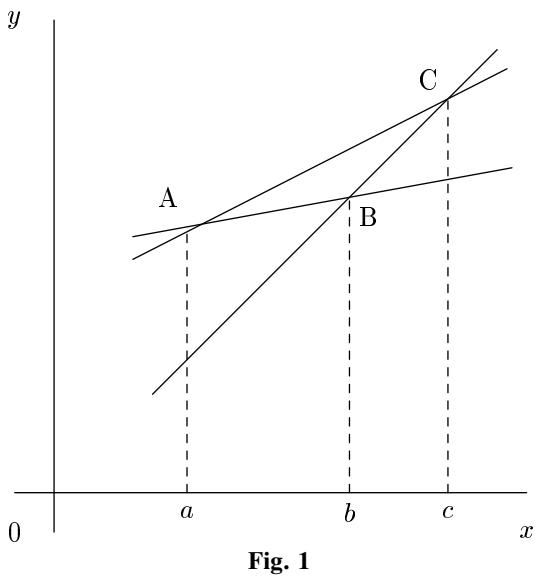
\includegraphics[keepaspectratio]{images/part001_7b60909a.jpg}}

\subsection{DEFINITION OF A CONVEX FUNCTION}

DEFINITION 1. We say that a finite numerical function \(f\) , defined on an interval \(\mathrm{I} \subset \mathbf{R}\) , is convex on \(\mathrm{I}\) if, no matter what the points \(x, x'\) of \(\mathrm{I}\) , \((x < x')\) , every point \(\mathrm{M}_z\) of the graph \(\mathrm{G}\) of \(f\) such that \(x \leqslant z \leqslant x'\) lies below the segment \(\mathrm{M}_x\mathrm{M}_{x'}\) (or, what comes to the same, if every point of this segment lies above \(\mathrm{G}\) ) (fig.~2).

\pandocbounded{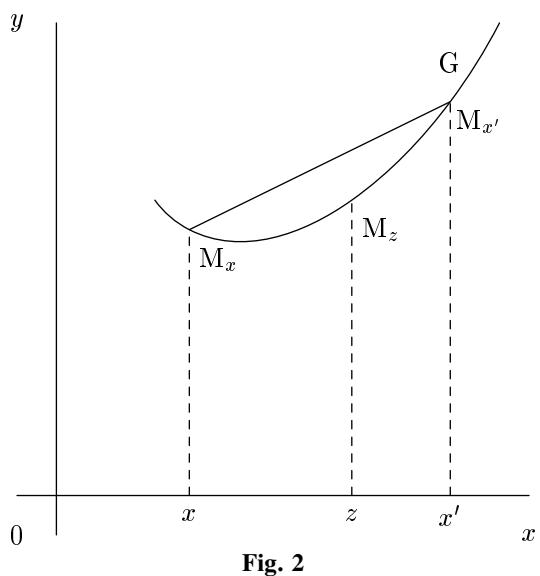
\includegraphics[keepaspectratio]{images/part001_0967d261.jpg}}

Taking account of the parametric representation of a segment (Gen.~Top., VI, p.~35), the condition for f to be convex on I is that one has the inequality

\[
f (\lambda x + (1 - \lambda) x ^ {\prime}) \leqslant \lambda f (x) + (1 - \lambda) f (x ^ {\prime})\tag{1}
\]

for each pair of points \((x, x')\) of I and every \(\lambda \in [0, 1]\) .

Definition 1 is equivalent to the following: the set of points in \(\mathbf{R}^2\) lying above the graph \(G\) of \(f\) is convex. Indeed, this condition is clearly sufficient for \(f\) to be convex on I; it is also necessary, for if \(f\) is convex on I, and if \((x,y)\) , \((x',y')\) are two points lying above \(G\) , then one has \(y \geqslant f(x)\) , \(y' \geqslant f(x')\) , from which, for \(0 \leqslant \lambda \leqslant 1\) ,

\[
\lambda y + (1 - \lambda) y ^ {\prime} \geqslant \lambda f (x) + (1 - \lambda) f \left(x ^ {\prime}\right) \geqslant f (\lambda x + (1 - \lambda) x ^ {\prime})
\]

by (1), which shows that every point of the segment with endpoints \((x, y)\) and \((x', y')\) lies above G.

Remark. On sees in the same way that the set of points lying strictly above G is convex. Conversely, if this set is convex one has

\[
\lambda y + (1 - \lambda) y ^ {\prime} > f (\lambda x + (1 - \lambda) x ^ {\prime})
\]

for \(0 \leqslant \lambda \leqslant 1\) and \(y > f(x)\) , \(y' > f(x')\) ; on letting \(y\) tend to \(f(x)\) and \(y'\) approach \(f(x')\) in this formula it follows that \(f\) is convex.

Examples. 1) Every (real) affine linear function \(ax + b\) is convex on \(\mathbf{R}\) .

\begin{enumerate}
\def\labelenumi{\arabic{enumi})}
\setcounter{enumi}{1}
\tightlist
\item
  The function \(x^{2}\) is convex on \(\mathbf{R}\) , since one has
\end{enumerate}

\[
\lambda x ^ {2} + (1 - \lambda) x ^ {\prime 2} - \left(\lambda x + (1 - \lambda) x ^ {\prime}\right) ^ {2} = \lambda (1 - \lambda) (x - x ^ {\prime}) ^ {2} \geqslant 0
\]

for \(0 \leqslant \lambda \leqslant 1\) .

\begin{enumerate}
\def\labelenumi{\arabic{enumi})}
\setcounter{enumi}{2}
\tightlist
\item
  The function \(|x|\) is convex on \(\mathbf{R}\) , since
\end{enumerate}

\[
\left| \lambda x + (1 - \lambda) x ^ {\prime} \right| \leqslant \lambda | x | + (1 - \lambda) \left| x ^ {\prime} \right|
\]

for \(0 \leqslant \lambda \leqslant 1\) .

It is clear that if \(f\) is convex on \(\mathbf{I}\) , then its restriction to any interval \(\mathbf{J} \subset \mathbf{I}\) is convex on \(\mathbf{J}\) .

Let \(f\) be a convex function on \(I\) , and \(x, x'\) two points of \(I\) such that \(x < x'\) ; if \(z \in I\) is exterior to \([x, x']\) then \(M_z\) lies above the line \(D\) joining \(M_x\) and \(M_{x'}\) ; this is an immediate consequence of the lemma.

One deduces from this that if z is a point such that \(x < z < x'\) and such that \(M_{z}\) lies on the segment \(M_{x}M_{x'}\) , then, for every other point \(z'\) such that \(x < z' < x'\) the point \(M_{z'}\) also lies on the segment \(M_{x}M_{x'}\) , for it follows from the above that \(M_{z'}\) is at the same time both above and below this segment; in other words, f is then equal to an affine linear function on \([x, x']\) .

DEFINITION 2. We say that a finite real function \(f\) defined on an interval \(\mathbf{I} \subset \mathbf{R}\) is strictly convex on \(\mathbf{I}\) if, for any points \(x, x'\) of \(\mathbf{I}\) ( \(x < x'\) ), every point \(\mathbf{M}_z\) of the graph \(\mathbf{G}\) of \(f\) such that \(x < z < x'\) lies strictly below the segment \(\mathbf{M}_x\mathbf{M}_{x'}\) (or, what comes to the same, if every point of the segment, apart from the endpoints, lies strictly above \(\mathbf{G}\) ).

In other words, we must have the inequality

\[
f (\lambda x + (1 - \lambda) x ^ {\prime}) <   \lambda f (x) + (1 - \lambda) f (x ^ {\prime})\tag{2}
\]

for every pair of distinct points \((x, x')\) of I and every \(\lambda\) such that \(0 < \lambda < 1\) .

The remarks that precede def. 2 show that for a convex function f to be strictly convex on I it is necessary and sufficient that there be no interval contained in I (not reducing to a single point) such that the restriction of f to this interval is affine linear.

Of the examples above, the first and third are not strictly convex; on the other hand, \(x^2\) is strictly convex on \(\mathbf{R}\) ; a similar calculation shows that \(1 / x\) is strictly convex on \(]0, +\infty[\) .

PROPOSITION 1. Let \(f\) be a finite real function, convex (resp. strictly convex) on an interval \(\mathbf{I} \subset \mathbf{R}\) . For every family \((x_i)_{1 \leqslant i \leqslant p}\) of \(p \geqslant 2\) distinct points of \(\mathbf{I}\) , and every family \((\lambda_i)_{1 \leqslant i \leqslant p}\) of \(p\) real numbers such that \(0 < \lambda_i < 1\) and \(\sum_{i=1}^{p} \lambda_i = 1\) , we have

\[
f \left(\sum_ {i = 1} ^ {p} \lambda_ {i} x _ {i}\right) \leqslant \sum_ {i = 1} ^ {p} \lambda_ {i} f (x _ {i})\tag{3}
\]

(resp.

\[
f \left(\sum_ {i = 1} ^ {p} \lambda_ {i} x _ {i}\right) <   \sum_ {i = 1} ^ {p} \lambda_ {i} f (x _ {i})).\tag{4}
\]

Since the proposition (for convex functions) reduces to the inequality (1) for \(p = 2\) we argue by induction for \(p > 2\) . The number \(\mu = \sum_{i=1}^{p-1} \lambda_i\) is \(> 0\) ; it is immediate that if \(a\) and \(b\) are the smallest and largest of the \(x_i\) then \(a \leqslant \sum_{i=1}^{p-1} \lambda_i x_i / \sum_{i=1}^{p-1} \lambda_i \leqslant b\) ; in other words, the point \(x = \frac{1}{\mu} \sum_{i=1}^{p-1} \lambda_i x_i\) belongs to I, and the induction hypothesis implies that \(\mu f(x) \leqslant \sum_{i=1}^{p-1} \lambda_i f(x_i)\) ; moreover we have, from (1), that

\[
f \left(\sum_ {i = 1} ^ {p} \lambda_ {i} x _ {i}\right) = f (\mu x + (1 - \mu) x _ {p}) \leqslant \mu f (x) + (1 - \mu) f (x _ {p}) \leqslant \sum_ {i = 1} ^ {p} \lambda_ {i} f (x _ {i}).
\]

One argues in the same way for strictly convex functions, starting from the inequality (2).

We say that a finite real function \(f\) is concave (resp. strictly concave) on I if \(-f\) is convex (resp. strictly convex) on I. It comes to the same to say that for every pair \((x, x')\) of distinct points of I and every \(\lambda\) such that \(0 < \lambda < 1\) one has

\[
f (\lambda x + (1 - \lambda) x ^ {\prime}) \geqslant \lambda f (x) + (1 - \lambda) f (x ^ {\prime})
\]

\[
(\text { resp. } f (\lambda x + (1 - \lambda) x ^ {\prime}) > \lambda f (x) + (1 - \lambda) f (x ^ {\prime})).
\]

\subsection{FAMILIES OF CONVEX FUNCTIONS}

PROPOSITION 2. Let \(f_{i}\) ( \(1 \leqslant i \leqslant p\) ) be \(p\) convex functions on an interval \(\mathbf{I} \subset \mathbf{R}\) , and \(c_{i}\) ( \(1 \leqslant i \leqslant p\) ) be \(p\) arbitrary positive numbers; then the function \(f = \sum_{i=1}^{p} c_{i} f_{i}\) is convex on \(\mathbf{I}\) . Further, if for at least one index \(j\) the function \(f_{j}\) is strictly convex on \(\mathbf{I}\) , and \(c_{j} > 0\) , then \(f\) is strictly convex on \(\mathbf{I}\) .

This follows immediately by applying the inequality (1) (resp. (2)) to each of the \(f_{i}\) , multiplying the inequality for \(f_{i}\) by \(c_{i}\) , and then adding term-by-term.

PROPOSITION 3. Let \((f_{\alpha})\) be a family of convex functions on an interval \(\mathbf{I} \subset \mathbf{R}\) ; if the upper envelope \(g\) of this family is finite at every point of \(\mathbf{I}\) then \(g\) is convex on \(\mathbf{I}\) .

Indeed, the set of points \((x, y) \in \mathbf{R}^{2}\) lying above the graph of g is the intersection of the convex sets formed by the points lying above the graph of each of the functions \(f_{\alpha}\) ; so it is convex.

PROPOSITION 4. Let H be a set of convex functions on an interval \(I \subset R\) ; if F is a filter on H which converges pointwise on I to a finite real function \(f_{0}\) , then this function is convex on I.

To see this it suffices to pass to the limit along F in the inequality (1).
